\documentclass[float=false, crop=true]{standalone}

\usepackage{tikz}
\usepackage{graphicx}

\usetikzlibrary{automata, positioning, arrows.meta}                             % Tikz macros

\begin{document}
\resizebox{0.45\columnwidth}{!}{%
  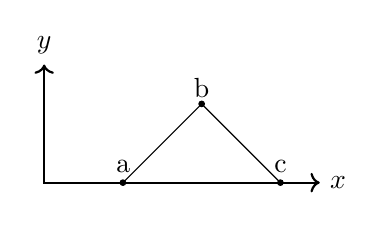
\begin{tikzpicture}[scale=1]    % Draw axes
    \draw [<->,thick] (0,1.5) node (yaxis) [above] {$y$}
    |- (3.5,0) node (xaxis) [right] {$x$};
    % Draw two intersecting lines
    \draw (1,0) coordinate (a_1) -- (2,1) coordinate (a_2);
    \draw (3,0) coordinate (b_1) -- (2,1) coordinate (b_2);

    \filldraw [black] (a_1) circle (1pt);
    \filldraw [black] (a_2) circle (1pt);
    \filldraw [black] (b_1) circle (1pt);

    \node[yshift=0.2cm] at (a_1) {a};
    \node[yshift=0.2cm] at (a_2) {b};
    \node[yshift=0.2cm] at (b_1) {c};
  \end{tikzpicture}%
}

\end{document}
